\documentclass{beamer}
\graphicspath{ {graphics/}}
\begin{document}
\title{Literary Worlds Javascript Client}
\author{John Lewis, Owen Watson, Tim Cunningham}
\usenavigationsymbolstemplate{}
\frame{\titlepage}
\frame{\frametitle{Table of contents}\tableofcontents}

\section{Overview}
\frame{\frametitle{Overview} 
Literary Worlds is an multiuser text based game used for English education at WMU.\\
Most of these text based games provide a telnet interface for playing, Literary Worlds uses MOOTcan, a Java applet.\\
The aim of this project is to provide a drop-in replacement user interface in Javascript.\\
}

\section{Background}
\frame{\frametitle{Background}


}

\section{enCore}
\frame{\frametitle{enCore}
enCore is an graphical interface and MUD database package that works with a LambdaMOO server to provide a browser based text client as well as a graphical, mouse driven interface.
\\
The Java applet is the text interface, it makes a raw TCP connection (eg, telnet) to LambdaMOO, as though the user were using a command line telnet client.
}


\section{Xpress interface}
\frame{\frametitle{enCore Xpress interface}
\begin{centering}
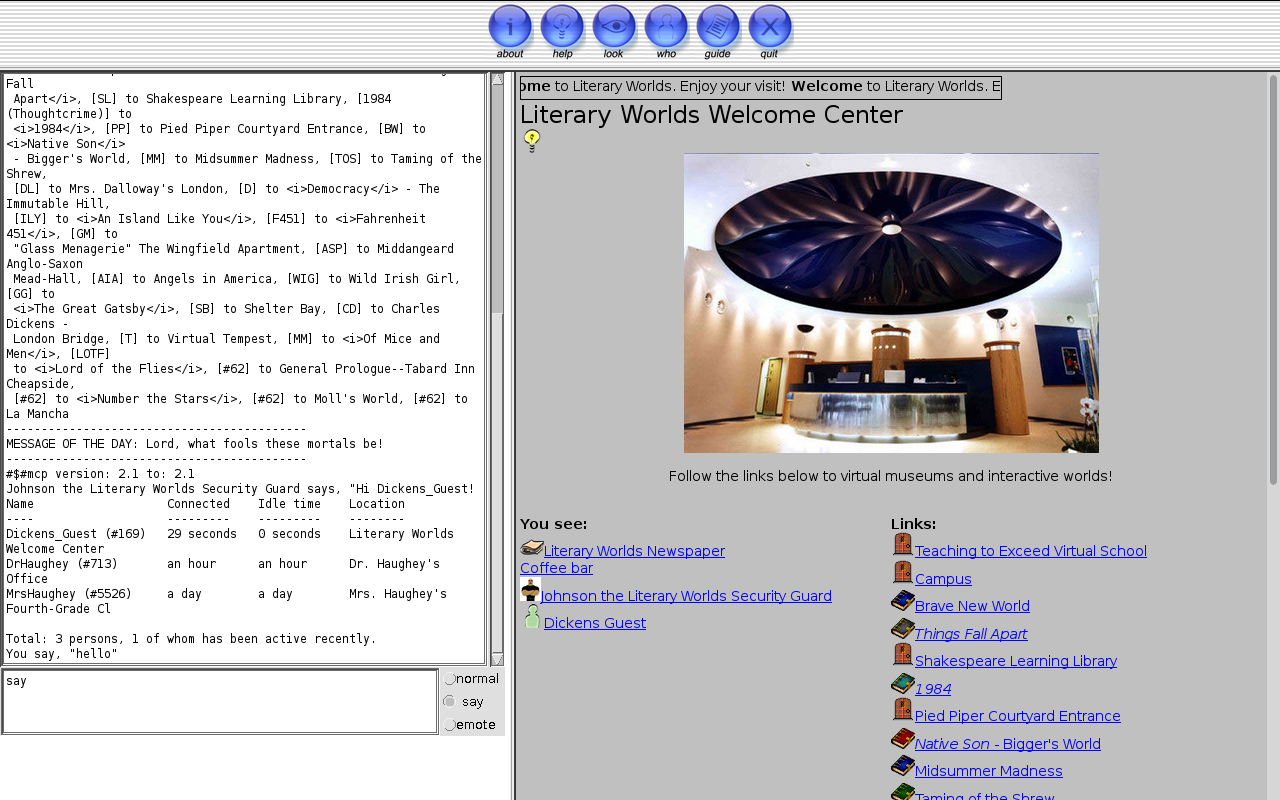
\includegraphics[width=\textwidth,height=\textheight,keepaspectratio]{classUsage.png}
\end{centering}
}

\section{Telnet and Browsers}
\frame{\frametitle{Providing raw TCP in client Javascript}
It is not possible to initiate a raw TCP connection in clientside Javascript, unlike Java applets.\\
Therefore, we need an intermediary server to connect over TCP, as well as to the browser client, and send data back and forth between the two.\\
This server must also support multiple concurrent users and handle asynchronous tasks and events.

}

\end{document}
